% !TeX program = XeLaTeX
% !TeX encoding = UTF-8
\documentclass[a4paper,oneside,12pt]{book}
\newcommand{\thesistitle}{A mobile exam proctoring system with deep-learning-based human action recognition} % Your thesis title, this is used in the title and abstract
\newcommand{\degree}{Master of Science in Computer Science \\ (Future Networked Systems)} % Your degree name, this is used in the title page and abstract
\newcommand{\typeofthesis}{dissertation} % dissertation, Final Year Project, report, etc.
\newcommand{\authorname}{Tong Ge} % Your name, this is used in the title page and PDF stuff
\newcommand{\supervisor}{Dr. Ciarán Mc Goldrick} 
%% Do not put your Student ID in the document, as TCD will not publish
%% documents that contain both your name and your Student ID.

\newcommand{\keywords}{Deep learning, pose-based features, video data, classification, mobile device, exam proctoring} % Keywords for your thesis
\newcommand{\school}{\href{http://www.scss.tcd.ie}{School of Computer Science and Statistics}} % Your school's name and URL, this is used in the title page

%% Comment out the next line if you don't want a department to appear
%\newcommand{\department}{\href{http://researchgroup.university.com}{Department Name}} % Your research group's name and URL, this is used in the title page

\AtBeginDocument{
\hypersetup{pdftitle=\thesistitle} % Set the PDF's title to your title
\hypersetup{pdfauthor=\authorname} % Set the PDF's author to your name
\hypersetup{pdfkeywords=\keywords} % Set the PDF's keywords to your keywords
}

%% Language and font encodings
% \usepackage[T1]{fontenc}
%\usepackage[utf8]{inputenc}
\usepackage[british]{babel}
\usepackage{fontspec}
\usepackage{xeCJK}
\setCJKmainfont{IPAMincho}
\setCJKsansfont{IPAGothic}
\setCJKmonofont{IPAGothic}
\usepackage{microtype}
%% Bibliographical stuff
% \usepackage[sort,comma,numbers]{natbib}
\usepackage[style=numeric, bibencoding=utf8, natbib=true, backend=biber, sorting=none]{biblatex}
\setcounter{biburllcpenalty}{7000}
\setcounter{biburlucpenalty}{8000}
%% Document size
% include showframe as an option if you want to see the boxes
\usepackage[a4paper,top=2.54cm,bottom=2.54cm,left=3cm,right=1.8cm,headheight=16pt]{geometry}
\setlength{\marginparwidth}{2cm}
\usepackage{url}
\urlstyle{sf}
\Urlmuskip=0mu plus 10mu
\usepackage[nottoc]{tocbibind}
%% Useful packages
\usepackage{float}
\usepackage[newfloat]{minted}
\usepackage{amsmath}
\usepackage[strict,autostyle=true]{csquotes} % Required to generate language-dependent quotes in the bibliography
\usepackage{graphicx}
\usepackage[usenames,dvipsnames,svgnames,table,xcdraw]{xcolor}
\usepackage{psfrag,wrapfig}
\usepackage[colorinlistoftodos]{todonotes}
\usepackage[colorlinks=true, allcolors=black]{hyperref}
\usepackage{caption} % if no caption, no colon
\usepackage[ruled,vlined,linesnumbered,resetcount,algochapter]{algorithm2e}
\usepackage{sfmath} %use sans-serif in the maths sections too
\usepackage[parfill]{parskip}    % Begin paragraphs with an empty line rather than an indent
\usepackage{setspace} % to permit one-and-a-half or double spacing
\usepackage{enumerate} % fancy enumerations like (i) (ii) or (a) (b) and suchlike
\usepackage{booktabs} % To thicken table lines
\usepackage{titletoc}
\usepackage{color}
\usepackage{multirow,multicol}
\usepackage{supertabular}
\usepackage{tabularx}
\usepackage{ltxtable}
\usepackage{fancyhdr}
\usepackage{pdflscape}
\usepackage{mathtools}
\DeclarePairedDelimiter\ceil{\lceil}{\rceil}
\DeclarePairedDelimiter\floor{\lfloor}{\rfloor}

\pagestyle{plain}
%% It is not a requirement of the university that the font should be sans-serif, but
%% the Mechanical engineers require it. Comment out the following line to disable it
% \renewcommand{\familydefault}{\sfdefault} %use the sans-serif font as default

%% If you're not using sans-serif, consider using Palatino instead of the LaTeX standard
\usepackage{mathpazo} % Use the Palatino font by default if you prefer it to Computer Modern
\setmainfont
     [ BoldFont       = texgyrepagella-bold.otf ,
       ItalicFont     = texgyrepagella-italic.otf ,
       BoldItalicFont = texgyrepagella-bolditalic.otf ]
     {texgyrepagella-regular.otf}

\renewcommand{\theequation}{\arabic{equation}} %% use continuous equation numbers

%% Format Chapter headings appropriately
\usepackage{titlesec}
\titleformat{\chapter}[hang]
{\normalfont\huge\bfseries}{\thechapter}{1cm}{} 

\def\changemargin#1#2{\list{}{\rightmargin#2\leftmargin#1}\item[]}
\let\endchangemargin=\endlist

\newenvironment{abstract}%
    {\begin{center}%
    \bfseries{Abstract} \end{center}}
    
\usepackage{lipsum}
% \usepackage{draftwatermark}
% \SetWatermarkText{DRAFT}
% \SetWatermarkScale{1}
\newcommand*{\eqcite}[1]{%
  \vadjust{%
    \smallskip
    \hbox to \linewidth{\hfill\citet{#1}}%
  }%
}
\numberwithin{equation}{chapter}
    
\titlecontents{chapter}
[0pt]             % left margin
{\vspace{4pt}}    % above code
{\textsc{\bfseries\thecontentslabel.}~}
{}             % unnumbered format
{\titlerule*[6pt]{}\contentspage}
\titlecontents{section}
[.5cm]             % left margin
{\vspace{4pt}}    % above code
{{\bfseries\thecontentslabel}~} % numbered format
{}             % unnumbered format
{\titlerule*[6pt]{.}\contentspage}
\titlecontents{subsection}
[1.2cm]             % left margin
{\vspace{4pt}}    % above code
{{\bfseries\thecontentslabel}~} % numbered format
{}             % unnumbered format
{\titlerule*[6pt]{.}\contentspage}
\title{\thesistitle}
\author{\authorname}

\addbibresource{bibs/background.bib}
\addbibresource{bibs/prevResearch.bib}
\addbibresource{bibs/deepModel.bib}
\addbibresource{bibs/mobileOptimus.bib}
\addbibresource{bibs/impletEval.bib}

\frontmatter
\begin{document}
\addtocontents{toc}{\vspace*{-1cm}}
\begin{titlepage}

\center % Center everything on the page

%% All the text parameters should be taken from the start of the main.tex file.
%% You should only alter stuff here if you want to change the layout

%----------------------------------------------------------------------------------------
%	LOGO SECTION
%----------------------------------------------------------------------------------------
%% Choose one of the following -- a colour or black-and-white logo


\includegraphics{title/Trinity_RGB_transparent_main.png}\\[1cm] 
%
\includegraphics[width=12cm]{title/black-stacked-trinity.jpg}\\[1cm] 

\Large \school\\[1.5cm] % Minor heading such as course title
\ifdefined\department
\large \department\\[1.5cm] % Minor heading such as course title
\fi

%----------------------------------------------------------------------------------------
%	TITLE SECTION
%----------------------------------------------------------------------------------------
\makeatletter
{ \huge \bfseries \thesistitle}\\[1.5cm] % Title of your document
 

%----------------------------------------------------------------------------------------
%	AUTHOR SECTION
%----------------------------------------------------------------------------------------

\ifdefined\authorid
\authorname\\ % Your name
\authorid\\[2cm] % Your Student ID
\else
\authorname\\[2cm] % Your name
\fi

%----------------------------------------------------------------------------------------
%	DATE SECTION
%----------------------------------------------------------------------------------------

{\large \today}\\[2cm] % Date, change the \today to a set date if you want to be precise

 
%----------------------------------------------------------------------------------------
%	TYPE OF THESIS SECTION
%----------------------------------------------------------------------------------------
\vfill
 A \typeofthesis\ submitted in partial fulfilment\\of the requirements for the degree of\\
\degree

\vfill % Fill the rest of the page with whitespace

\end{titlepage}
\pagenumbering{roman}
\chapter*{\Huge{Declaration}}
\vspace{1cm}
I hereby declare that this \typeofthesis\ is entirely my own work and that it has not been submitted as an exercise for a degree at this or any other university.

\vspace{1cm}
I have read and I understand the plagiarism provisions in the General Regulations of the University Calendar for the current year, found at \url{http://www.tcd.ie/calendar}.
\vspace{1cm}

I have also completed the Online Tutorial on avoiding plagiarism `Ready Steady Write', located at \url{http://tcd-ie.libguides.com/plagiarism/ready-steady-write}.
\vspace{1cm}

I agree that Trinity College Library may lend or copy this dissertation upon request.
\vspace{3cm}

Signed:~\rule{5cm}{0.3pt}\hfill Date:~\rule{5cm}{0.3pt}
\begin{figure}[h!]
    \vspace*{-1.4cm}
    \hspace{2cm}
    
\includegraphics{title/sign.pdf}
\end{figure}
\newpage
\newpage
\vspace*{1cm}
\begin{center}
\linespread{1.3}
\selectfont
\huge \bfseries \thesistitle\\[1cm]
\end{center}
\begin{center}
\authorname, \degree\\
University of Dublin, Trinity College, 2021\\
Supervisor: \supervisor
\end{center}
\vspace*{1cm}
\phantomsection
\addcontentsline{toc}{chapter}{Abstract}
\begin{abstract}
\begin{changemargin}{1cm}{1cm}
The COVID-19 pandemic has prevented students from congregating to take traditional in-person exams, shifting the attention of pedagogical institutions to online exam systems accessed remotely. 
This research surveys previous review papers on human action recognition to confirm the feasibility of obtaining action features from spatiotemporal data sets such as videos.
This research reviews multiple state-of-the-art deep models and optimisation methods under the premise of achieving a balance between performance, function and resource demand constraints of mobile devices.
Then a deep learning model is developed to classify the behaviour of examinees to a series of activities, approved or prohibited by the exam holder.
The model evaluation carefully considers the model performance in machine learning classification metrics and computational performance.
Experimental results show that the proposed model achieved over 90\% accuracy over 12 exam-related action categories with 23.6M parameters, making it possible to run inference smoothly on most modern mobile phones.
Finally, this research concludes with a discussion of model design and optimisation experiences with possible directions for future research in this area.

\vspace{1cm}
\begin{flushleft}
   \let\and\\%
   \textbf{Keywords:} \keywords
\end{flushleft}
\end{changemargin}
\end{abstract}

\newpage
\chapter{Acknowledgements}
{
\linespread{1.3}
\selectfont
First and foremost, I would like to express my profound gratitude to my supervisor Associate Professor Ciarán Mc Goldrick, who has provided me with constant support and guidance through each stage of this dissertation. Through his strict guidance and gentle encouragement from time to time, I can personally feel my weakness and the direction of my future efforts.

I am deeply grateful to Trinity College Dublin and the School of Computer Science and Statistics for teaching me the theoretical foundation, practical techniques of computer science and innovative research methods. In addition, the use of web hosting services and the support of computing power have provided great help for data collection and model training in this research.

Last but not least, I am truly thankful to my solicitous parents for their warm regards and financial supports for studying abroad and upholding my chosen academic path.

\vspace{1.2cm}
\begin{flushleft}
Tong Ge

\textit{University of Dublin, Trinity College Dublin \\
August 2021}
\end{flushleft}
}
\clearpage

\tableofcontents
\newpage
% \makeatletter
% \let\savedchap\@makeschapterhead
% \def\@makeschapterhead#1#2{\vspace*{-.5cm}\savedchap{#1}{#2}\vspace*{-.5cm}}
\listoffigures
% \let\@makeschapterhead\savedchap
% \makeatother
\listoftables
\begingroup
\let\clearpage\relax
\listofalgorithms
\addcontentsline{toc}{chapter}{List of Algorithms}
\endgroup
\newpage
\makeatletter
\let\mcnewpage=\newpage
\newcommand{\TrickSupertabularIntoMulticols}{%
  \renewcommand\newpage{%
    \if@firstcolumn
      \hrule width\linewidth height0pt
      \columnbreak
    \else
      \mcnewpage
    \fi
  }%
}
\makeatother
\chapter{Nomenclature}
\begin{changemargin}{-0.5cm}{0cm}
\begin{multicols*}{2}
\TrickSupertabularIntoMulticols
\begin{supertabular}{>{\em}lp{6.2cm}}
AuC & Area under the Curve (ROC Curve) \\ [.5em]
BotNet & Bottleneck Transformer \\ [.5em]
CNN & Convolutional Neural Network \\ [.5em]
GRU & Gated Recurrent Unit \\ [.5em]
LSTM & Long Short-Term Memory \\ [.5em]
R-CNN & Region-based Convolutional Neural Networks \\ [.5em]
ResNet & Residual neural Network \\ [.5em]
RNN & Recurrent Neural Network \\ [.5em]
ROC & Receiver Operating Characteristic \\ [.5em]
SVM & Support vector machines \\ [.5em]
VGG & Visual Geometry Group \\ [.5em]
ViT & Vision Transformer \\ [.5em]
YOLO & An object detection model abbreviated from You Only Look Once \\ [.5em]
\end{supertabular}
\end{multicols*}
\end{changemargin}

\mainmatter
\onehalfspacing
\chapter{Introduction}
\label{chap:Introduction}
This chapter introduces the background \ref{sec:Research background} of the current COVID-19 pandemic, leading to the research questions and aims \ref{sec:Research aims} to be achieved in this research.
Furthermore, since human participants are involved in data collection and model training, research ethics \ref{sec:Research ethics} are discussed. Finally, this chapter also presents the overview and structure \ref{sec:Dissertation overview} of this dissertation.
\section{Research background}
\label{sec:Research background}
%2 pages
%COVID-19 impacts education
COVID-19 has brought many challenges to higher education.
\citet{marinoni2020impact} reiterate the facts released by UNESCO regarding the significant impact of the pandemic on education in countries around the world.
For example, there are approximately 130 million students, accounting for 89.4\% of total enrolled learners, whose academic career has been vitiated because of the impact of pervading virus caused school closures.

To better respond to the crisis and allay public concerns caused by the epidemic, the International Association of Universities (IAU) launches a survey of the impact of COVID-19 on higher education.
\citet{marinoni2020impact} present the survey results showing that COVID-19 has inevitably affected many processes in education, including teaching \& learning, researching, and assessment.

In teaching and learning, most classroom lectures have been substituted by distance teaching and learning, which may not be difficult for professors and students who are familiar with computers and the Internet.
On the other hand, experiments and research that require the use of shared professional equipment are much more severely affected.
The survey shows that 80\% of researchers have reported that their research progress is decelerating and moving at a creep.

However, as for assessment and examination, institutions have no way to perpetuating the traditional assessment methods, which is indicated by \citet{clark2020testing} as one of the most important challenges for students.
``Learning assessment and examination approaches will be reviewed, and institutions may choose to invest further in technical infrastructures'', said by \citet{marinoni2020impact} points out the fact.
Although some universities shift from closed-book exams to pure continuous assessments immediately, other educational institutions are craving for new technologies to help them out of trouble.

As a result, the motivation of this research is to investigate the feasibility of deep-learning-based human action recognition techniques in the distance invigilation application and provide a way for educational institutions to hold exams and reduce labour costs.

%Deep learning technologies are widely used, applications
In recent years, ubiquitous influences of deep learning methods have brought tremendous advancement to many computer science fields and individual's daily life. 
In many fields, such as computer vision and natural language processing, deep learning approaches achieved higher performance than traditional algorithms.
\citet{mccay2020abnormal} show that in the research field of automatic human action recognition, the analysis and reconstruction of human actions have copious applications, including content-based video indexing, intelligent surveillance, human-computer interaction, and virtual reality.
Therefore, this research will explore deep learning techniques to solve automatic exam invigilation problems in the assessment process of distance education.

This research is also based on previous studies in deep learning and deep model mobilisation.
Currently, there are some existing models for human posture analysis and detection.
But many of them use static imagery as input and key points of the body as output, and they are not optimised for mobile devices with limited computing power.
Beside, the personal computer hardware, the bridge between the software system and the physical space, is not trusted.
However, a trusted software environment can be ensured on mobile phones with hardware attestation functions provided by operating system and device manufactures.


\section{Research aims}
\label{sec:Research aims}
%1 page
After clarifying the research background, the research question of this dissertation is summarised as the following:

\begin{quote}
    Is it possible to understand sequential human actions from an on-device camera video input stream with deep learning technologies to classify the series of actions of the exam attendee to approved or prohibited behaviours with high accuracy?
\end{quote}

In order to answer the research question, this research aims to achieve the objectives through the corresponding methods shown in Table \ref{tab:Research objectives}.

\begin{table}[!ht]
    \centering
    \begin{longtable}{>{\hspace*{-0.3cm}$\bullet$\hspace*{0.2cm}}p{.4\textwidth}p{.56\textwidth}}
\textbf{Research objectives} & \textbf{Method to achieve objectives} \\ \hline
To do the literature review & By surveying the state-of-the-art technologies of deep-learning-based human action recognition \\ \hline
To have an available data set & By obtaining a suitable image and video data set and labelling them for training the model \\ \hline
To design a deep learning model & By designing a deep learning model \\ \hline
To code and train the deep model & By training the model and fine-tuning hyper-parameters \\ \hline
To optimise the model for mobile & By developing a working mobile app that equips the model \\ 
\end{longtable}
    \caption{Research objectives and corresponding methods}
    \label{tab:Research objectives}
\end{table}

After completing the above objectives, this research will also evaluate the project outcomes, especially for model performance and other following aspects.

\begin{itemize}
    \item Model accuracy, precision and other evaluation metrics on the classification task.
    \item Balanced performance between accuracy and efficiency of the deep learning model.
    \item User experiences of the overall system.
\end{itemize}


\section{Research ethics}
\label{sec:Research ethics}
%2 pages

\section{Dissertation overview}
\label{sec:Dissertation overview}
%.5 page
This dissertation comprises six chapters, beginning with this introduction chapter \ref{chap:Introduction}, presenting the research background, aims and ethics, followed by the literature review chapter \ref{chap:Literature review}, which comprehensively reviews previous researches on deep learning models and the related state-of-the-art works.
In chapter \ref{chap:Design}, this dissertation proposes the deep learning model used to recognise and classify actions, based on various designing trade-offs and mobile optimisation methods learned from previous research.
Figure \ref{fig:0-Intro-Overview} shows the project overview, in which these process pipelines and the proposed deep learning model are implemented in chapter \ref{chap:Implementation}.
Further, the experiments are conducted

\begin{figure}[h]
    \centering
    \hspace*{-.5cm}
    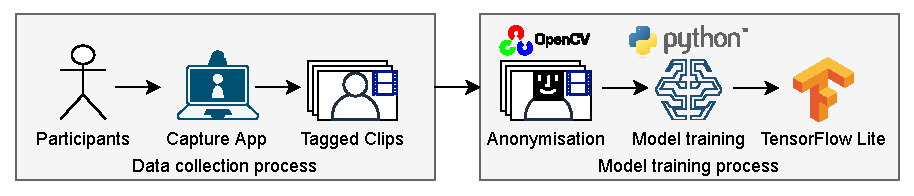
\includegraphics[scale=1.1]{introduction/imgs/0-Intro-Overview.pdf}
    \caption{Project overview}
    \label{fig:0-Intro-Overview}
\end{figure}
 % 4 pages
\chapter{Literature review}
\label{chap: Literature review}

\section{Traditional approaches}
\label{sec:Traditional approaches}
% 2 pages

\citet{schuldt2004recognizing}

\citet{gorelick2007actions}

\citet{marszalek2009actions}

\citet{Soomro2014} % 2 pages
\section{Deep learning-based methods}
\label{sec:Deep learning-based methods}
% 4 pages % 3 pages
\section{Online exam security system}
\label{sec:Online exam security system}
% 1 pages
In order to learn about the background of the security system of remote exams and propose a new system that better adapts to the status quo, this research reviews the previous research on the security system of online exams in this section.

Before the COVID-19 pandemic, the technology of paperless testing through computer systems has been widely used. For example, TOEFL iBT (Internet-based test) has gradually replaced the PBT (paper-based test) by using the Internet and computers for paperless exams from late 2005.
Another example is specific exams that are impossible to be sat on paper, such as programming competitions or exams requiring running compilers.
Although all these exams were in the form of using computers and the Internet, students were required to congregate in testing centers.

% Authentication
As a result, most of the previous research in this field assumes that the exam can still be organised in test centres, so the research direction of exam security focusing on biometric authentication.
For example, \citet{traore2017ensuring} propose a multi-modal biometric authentication framework, including face biometric and dynamic biometric from computer input devices, such as mouse and keyboard.
The purpose of biometric authentication is to prevent imposters in the exam, and the invigilators of the test centre should detect other cheating in time.

Nowadays, the pandemic segregates students at home for remote exams, invalidating the previous assumption.
There are still some studies proposing new solutions for biometric authentication in exams. 
In Japan, \citet{Akiko202144107} propose a new continuous biometric authentication method based on hand image features, which can prevent cheating, especially impersonation due to lack of invigilation. 
They use a mirror and a wide-angle lens to capture the images of students' hands when they take the exam and obtain the contour features of the hands through image processing.
However, any biometric authentication cannot prevent cheating by the students per se, such as using mobile phones to search online or seeking help from others.

In 2020, \citet{garg2020convolutional} point out that many security issues still exist in online exams, and propose a system based on Haar Cascade Classifier and Convolutional Neural Network to detect, track, tag, and identify the student's face.
Although this system innovatively uses deep learning models, only using facial features and constraints in the design is not comprehensive compared to action recognition.
And another disadvantage is focusing on facial features may cause contention in privacy risks mentioned in the research ethics section \ref{sec:Research ethics}.
For example, students can still cheat with mobile phones during online exams even with the facial-based security system enabled.

% confirm originality
After investigating many previous studies on online exam security systems, it is concluded that most of the research is limited to biometrics authentication, and there is no readily available security system that equips a deep-learning-based human action recognition model.
As a result, this research originally applied the human action recognition technique to the online exam security system.
 % 1.5 pages
\section{Deep models details}
\label{sec:Deep models details}
% 4 pages
\subsection{Convolutional neural network}
% 3DCNN
\subsection{Recurrent neural network}
% et optimus
\subsection{Attention and transformer}

\subsection{State-of-the-art models} % 4 pages
\section{Related works using deep models}
\label{sec:Related works using deep models}
% 4 pages
% review 0.5 page
\subsection{Human action recognition overview}
\citet{wu2017recent}

\citet{chen2020monocular}
 % 1 page

% 3DCNN %% Video related 1.5 page
\subsection{3D-CNN and RNN based methods}
\label{subsec: 3D-CNN and RNN based methods}
The standard two-dimensional convolution uses a two-dimensional kernel filter on each channel, and only two-dimensional features can be extracted.
\citet{tran2015learning} reviewed many previous 3-dimensional convolutional networks (3D-CNN) and highlighted relevant applications on spatiotemporal features in video dataset.
As shown in Figure \ref{fig:2-2dcnn-3dcnn}, 2D convolutional kernel filters are expanded to 3D and allow them running on multiple channels simultaneously.
3D-CNN is widely used in tasks that process multiple images at the same time, such as medical computed tomography (CT) scan data and video data.

\begin{figure}[!ht]
    \centering
    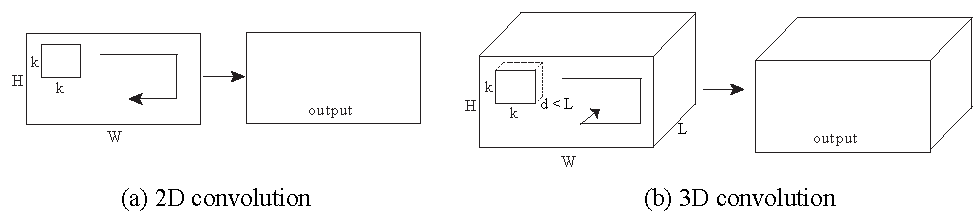
\includegraphics[width=\textwidth]{literature/imgs/2-2dcnn-3dcnn.pdf}
    \caption{2D convolution and 3D convolution \cite{tran2015learning}}
    \label{fig:2-2dcnn-3dcnn}
\end{figure}

The difference between the proposed 3D convolution and the multi-channel 2D convolution is that the 3D convolution uses weight-sharing kernel filters, while the multi-channel 2D convolutional kernel filters have different weights for each channel and ignore adjacent channels in computation.

Back to 2011, \citet{baccouche2011sequential} firstly applied a composed architecture of 3D convolution and RNN to the human action recognition task.
In this work, 3D convolution is firstly used for learning spatiotemporal features automatically, followed by an RNN `` to classify each sequence considering the temporal evolution of the learned features for each timestep'', said by \citet{baccouche2011sequential}.
The researchers also spotted the performance drawback of the RNN and will investigate the possibility of using a single-step model in future work.

One year after, \citet{ji20123d} proposed a human action recognition model composed purely of convolutional operations. %, as shown in Figure \ref{fig:ext-2-3dcnn-har}.
The premature network design is shallow and does not use residual connections, which are very similar in architecture to LeNet, consisting of multiple convolutional layers and pooling layers. In addition, they add some designed features (optical flow fields in many directions) to input, which is not an end-to-end trainable network.

% \begin{figure}[!ht]
%     \centering
%     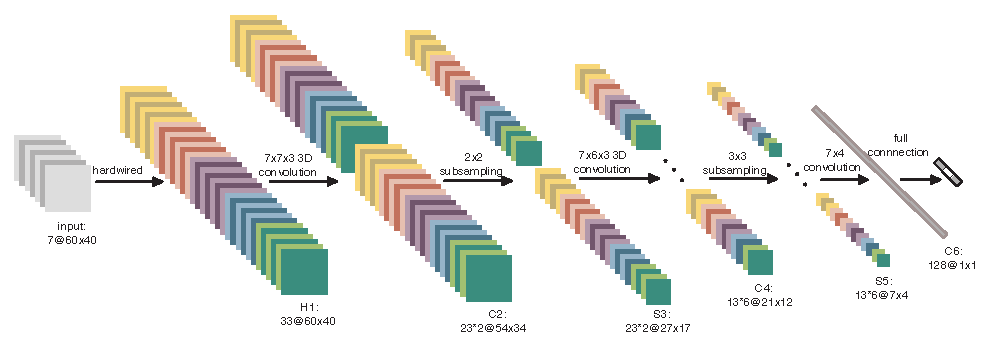
\includegraphics[width=\textwidth]{literature/imgs/ext-2-3dcnn-har.pdf}
%     \caption{A 3D-CNN model for human action recognition \cite{ji20123d}}
%     \label{fig:ext-2-3dcnn-har}
% \end{figure}

After several years of development, \citet{tran2015learning} proposed model Convolutional 3D (C3D) that achieved the state-of-the-art in video tasks in 2015.
This model does not involve the input of additional handcrafted features at all, but it also exposes some weaknesses of the 3D convolution.
For example, 3D-CNN cannot use pre-trained results from 2D images, such as ImageNet.
Also, the network has too many parameters, which is prone to over-fitting in the case of using an insufficient amount of video training data.

To overcome the weaknesses of using CNN or RNN individually, \citet{simonyan2014twostream} proposed a Two-Stream network.
The network consists of a spatial flow focused on each image frame and a temporal flow focused on the calculated optical flow.
Based on the idea of using the Two-Stream network, \citet{feichtenhofer2016convolutional} pointed out that the fusion process in the last Softmax layer caused losses and 3D convolution can perfectly fuse the spatiotemporal information in the convolutional layers.

In 2018, \citet{carreira2018quo} summarised the previous research on different methods used in the field of action recognition, which is also discussed in this subsection, namely ConvNet+LSTM (CNN+RNN), 3D ConvNets (3D-CNN) and Two-Stream network.
Based on these previous ideas, Inflated Two-Stream 3D ConvNets (I3D) is proposed and achieved good results on both HMDB-51 and UCF-101 data sets. % 1 page

\subsection{Transformer-based Neural Networks}

\citet{sun2019learning}

\citet{neimark2021video}

\begin{figure}[!ht]
    \centering
    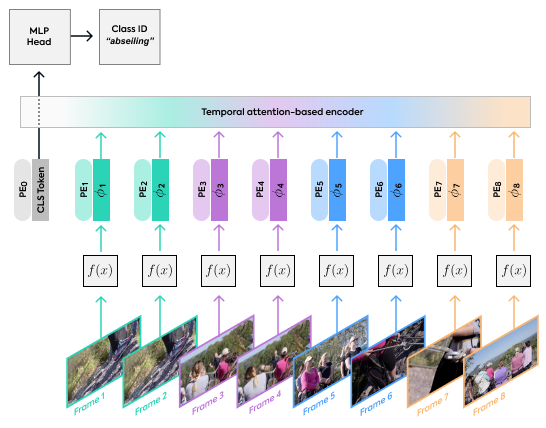
\includegraphics[width=.7\textwidth]{literature/imgs/ext-vtn.png}
    \caption{Video Transformer Network architecture \cite{neimark2021video}}
    \label{fig:ext-vtn}
\end{figure} % 2 page % 2 pages
\section{Mobile device optimisation}
\label{sec:Mobile device optimisation}
% 2 pages % 2 pages % 22 pages / 26
\chapter{Design}
 % 10 pages / 36
\chapter{Implementation}
\label{chap:Implementation}
% 8 pages
After designing the overall system, the next step is to program and implement the system.
In order to use simple and suitable technologies to efficiently develop and coding required system functions before writing the actual code, the first step will select technical frameworks and libraries to implement the system in section \ref{sec:Framework selection}.

After determining frameworks, the rest of this chapter will introduce three system modules, the data collection app developed with on web technology in section \ref{sec:Capture and data collection web app}, the implementation of the deep learning model and adapting the model to the mobile app on Android in section \ref{sec:Mobile application}.

\section{Framework selection}
\label{sec:Framework selection}
\subsection{Web development} %.5 page
\citet{nodejs2021}

\citet{react2021}

\citet{redux2021}

\subsection{Deep learning model development} %.5 page
%Tensorflow
\citet{abadi2015tensorflow}

%PyTorch
\citet{steiner2019pytorch}

\citet{florencio2019performance}

\subsection{Android application development} %1 page
% TFLite
\citet{singh2020mobile}

\citet{fadlilah2021development}

React Native \citet{eisenman2015learning} % 3.5 pages

\section{Data collection web app}
\label{sec:Data collection web app}
This section introduces several key user logics and algorithms in the data collection web application.
From the user's perspective, the data collection system mainly provides three user processes: new participant registration, participant login and the core function of participant recording and uploading, which are illustrated in Figure \ref{fig:4-webapp-user-register}, \ref{fig:4-webapp-user-login} and \ref{fig:4-webapp-user-record} respectively.

Figure \ref{fig:4-webapp-user-register} shows the registration process for new participants.
According to the research ethics, each participant needs to clearly understand the research content and provide consent before registering an account.
Another worth mentioning is that the system will generate a random password in the registration process and send it to the email provided by the registrant.
This registration process can prevent the system from collecting users' private passwords.

After the registration process, Figure \ref{fig:4-webapp-user-login} depicts the authentication process for registered participant.
The participant will input the email address and the random password received during the registration process.
If a participant forgot or lost the random password, he or she can request a new random password and restart the login process.

Figure \ref{fig:4-webapp-user-record} shows the main workflow of the data collection app after the participant logs in.
In the task selection stage, the web front-end first queries the currently available tasks from the back-end and display them in a list that participant can select.
Each task has detailed text and picture descriptions, which is easy for participants to understand.

After the participant selects desired tasks, the next step is video recording.
The system uses the web real-time communication (WebRTC\footnote{Real-time communication for the web: \url{https://webrtc.org/}}) API provided in most modern browsers to record videos for the participant.
Finally, in the upload step, participants can review each recorded videos and decide whether to upload or try rerecording.

The user registration and login process in the web app adopts a common secure authentication paradigm for online applications.
Algorithm \ref{algo:User authentication} displays the process of user authentication, where the password is double hashed and salted in back-end database storage.
In addition, the system uses short-term-valid JSON Web Tokens (JWT) as the access credentials for RPC calls, also incorporating the mechanism of a periodic token refresh, which further enhances system security and protects users' privacy.

\begin{minipage}{.5\textwidth}
\begin{algorithm}[H]
\caption{User authentication}
\label{algo:User authentication}
\KwData{Email $e$, Password $p$}
\KwResult{Auth $T_a$, Refresh $T_r$}
Web browser front-end:
$EP \gets concat(e, p)$
$h \gets sha256(EP)$
$send(e, h)$\;
\BlankLine
\BlankLine
\BlankLine
\BlankLine
Back-end:
$receive(e, h)$\;
\If{user $e$ does not exist}{
    return error\;
}
\If{bcrypt hash compare $h$ failed}{
    return error\;
}
\tcp{Authenticated}
$T_a \gets JWT(\{userDetail, authUUID\})$\;
$T_r \gets JWT(refreshUUID)$\;
return $T_a, T_r$\;
\end{algorithm}
\end{minipage}
\vline
\begin{minipage}{.5\textwidth}
\begin{algorithm}[H]
\caption{Video uploading}
\label{algo:Video uploading}
\KwData{Blob video data $v$}
\KwResult{Data in chunks $c[x]$}
$s \gets 3 \times 10^{4}$ \tcp*{gRPC 32768 bytes read limit}
\For{$i \gets 0$ \KwTo $\ceil*{\frac{sizeof(v)}{s}}$}{
    $b_{left} \gets i \times s$\;
    $b_{right} \gets \max ((i+1) \times s, sizeof(v))$\;
    $c[i] \gets v[b_{left}:b_{right}]$\;
    $send(i, c[i])$\;
    $progress \gets receive()$\;
    \If{receive progress failed}{
        return error\;
    }
    $updateUI(progress)$\;
    $i \gets i+1$\;
}
\end{algorithm}
\end{minipage}

Algorithm \ref{algo:Video uploading} shows the process for segmenting large video data before uploading it to the backend server.
This segmentation algorithm runs on the browser front end, using \textit{slice} in binary large object (Blob) API for slicing the video.
The communication between the front-end and back-end uses the gRPC bidirectional streaming.
When the front-end uploads data, it also receive acknowledgement and receiving progress from the server.
 % 2 pages

\section{Mobile app implementation}
\label{sec:Mobile app implementation}
After the data collection app is implemented, the data collection process begins.
While waiting for the data set to be collected, I designed the deep model as detailed in section \ref{sec:Deep model design}.
After the design of the model is completed, the data loader and the deep model are implemented using Python programming language and TensorFlow framework.
The implementation of EfficientNet (\textit{tf.keras.applications.efficientnet.EfficientNetB0}) and the MLP classification head (\textit{tf.keras.layers.Dense} and \textit{tf.keras.layers.Dropout}) is composed directly from the TensorFlow Keras-style high-level APIs.
The Longformer implementation uses the Hugging Face Transformer\footnote{Hugging Face Transformers: \url{https://huggingface.co/transformers/}} library.
The detail of each layer in the implemented model is shown in \ref{chap:Model design details}.
After finish implementing and training the deep model, the remaining research goal is to port the deep model to Android platform.

Although the most widely used programming language for Android development is Java, this project does not use Java except for the automatically generated initialisation codes and native function bindings.
As discussed in section \ref{sec:Framework selection}, the implementation uses React Native to develop UI and application logic.
Even though JavaScript development is more convenient, it is single-threaded and is not suitable for high performance parts in the application.
For the parts that require high performance, such as the image pipeline, the anonymisation process, and the deep model inference process, the C++ programming language is used for multi-threaded Android native development.

\subsection{Architecture overview}
The architecture of the mobile application developed in this research is shown in Figure \ref{fig:4-mobile-arch}.
The arrows in the figure indicate the direction of data flow and clearly show dependencies across different functional blocks.
The left half of the figure describes the user interface and user interaction logic developed using React Native, and the right half describes the core functions of the application developed using C++.
These two parts use React Native Javascript Interface (JSI) for communication.

\begin{figure}[!ht]
    \centering
    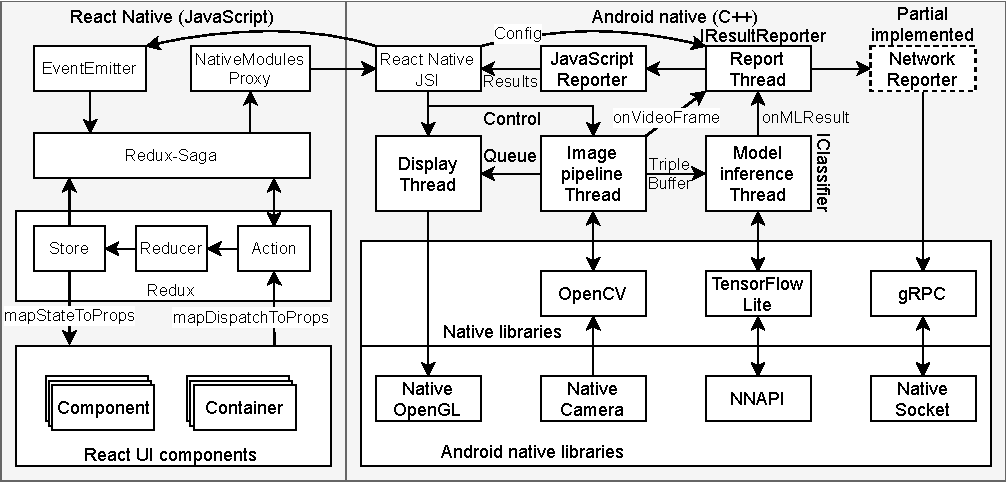
\includegraphics[width=\textwidth]{implementation/imgs/4-mobile-arch.pdf}
    \caption{Mobile app architecture and data flow}
    \label{fig:4-mobile-arch}
\end{figure}

The core functions of this project in the native part shown on the right side in Figure \ref{fig:4-mobile-arch} is much worth discussing than UI implementation on the left side.
These core functions include displaying images without lag and running model inference at the same time.
To achieve the goal, this project implements these functions in C++ by using multi-threading to enable asynchronous processing for display (a real-time task), model inference and network transmission (time-consuming tasks).
It can better take advantage of the multi-core of the mobile phone processor, and time-consuming tasks will not affect the real-time task, which ensures a smooth user experience.

\begin{figure}[!ht]
    \centering
    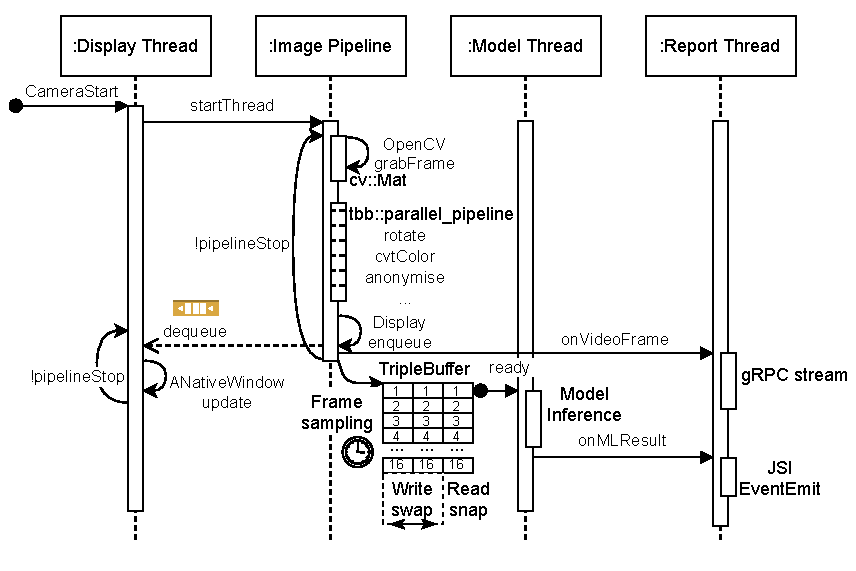
\includegraphics[width=\textwidth]{implementation/imgs/4-model-infer.pdf}
    \caption{Sequence diagram of the multi-threaded app}
    \label{fig:4-model-infer}
\end{figure}
The sequence diagram in Figure \ref{fig:4-model-infer} describes the interactions between four threads in the Android application.
After the user enters the exam screen, the display thread will receive the processed image data through a queue and update the display.
After the exam begins, the model inference thread will be started to receive processed image data from a triple buffer, and performs model inference, then informs the result report thread after getting the result.

The rest of this section will introduce in detail the multi-threaded design for the core function, including display thread, image processing pipeline thread, and model inference thread.

\subsection{Display and image processing pipeline}
This subsection introduces a real-time task involving the display and image processing pipeline in the app.
The image processing pipeline firstly receives an image from a camera on the mobile phone then transforms and anonymises it with OpenCV.
The display thread is responsible for receiving the image processed by the image processing pipeline and showing it through OpenGL.
This process is a real-time task, where the display process takes less time than the image processing process.
The display thread needs to wait for the processed image data from the processing pipeline thread.
Therefore, transferring data across two threads should use the producer-consumer programming paradigm with the blocking queue data structure.

A queue is a commonly used first-in-first-out (FIFO) data structure of a sequential organised collection of entities which can be modified by \textit{enqueue} (adding entities at one end) and \textit{dequeue} (removing entities from the other end).
A thread-safe blocking queue is a queue that may block in \textit{dequeue} operation or \textit{enqueue} operation.
If the blocking queue has already been empty, a \textit{dequeue} operation will block the calling thread until new data are available in the queue.
Conversely, a \textit{enqueue} operation will block the calling thread if the blocking queue has already full.

\begin{algorithm}[!ht]
\caption{Image processing pipeline thread}
\label{algo:Image processing pipeline thread}
\KwData{Readable image stream $v$ of cv::VideoCapture}
\KwResult{Processed image array $p$[] of cv::Mat}
initialisation\tcp*{OpenCV VideoCapture, CascadeClassifier, FacemarkLBF}
$STOP \gets false$\;
\While{not STOP}{
    $p_{bgr} \gets read(v)$\;
    $p_{grey} \gets cvtColor(p_{bgr}, BGR2GRAY)$\tcp*{Grey is used for detecting face}
    $p_{half} \gets resize(p_{grey}, 0.5f, 0.5f)$\tcp*{Scale down for better preformance}
    $p_{half} \gets equalizeHist(p_{half})$\tcp*{Histogram equalisation for better adaptation to different environmental lighting}
    $f$[] $\gets CascadeClassifier::detectMultiScale(p_{half}, parameters)$\;
    $l$[][] $\gets FacemarkLBF::fit(p_{half}, f$[]$)$\;
    \For{$i \gets 0$ \KwTo $sizeof\ f$[]}{
    $p_{anonymous} \gets drawCover(p_{bgr}, f$[$i$]$)$\;
    $p_{anonymous} \gets drawLandmark(p_{anonymous}, l$[$i$][]$)$\;
    }
    $p_{rgba} \gets cvtColor(p_{anonymous}, BGR2RGBA)$\tcp*{ANativeWindow requires image in RGBA format}
    $enqueue(displayQueue, p_{rgba})$\tcp*{Enqueue to display thread}
    $addImage(p_{anonymous})$\tcp*{Preform temporal sampling and add to the current writing queue in the triple buffer}
}
\end{algorithm}

Algorithm \ref{algo:Image processing pipeline thread} shows the simplified processing procedure in the image processing pipeline thread, which includes reading camera data, performing anonymisation, and sending the processed data to other threads.
For the display thread, it only needs to dequeue the RGBA data processed and converted by Algorithm \ref{algo:Image processing pipeline thread} from the $displayQueue$, and invoke the Android API to set the OpenGL texture.
In this way, the new frame will be displayed in real-time from the OpenGL rendering loop.

\subsection{Tensorflow Lite adoption and model inference}
Although Google provides some ready-made models and easy-to-call Java bindings, it is necessary to use C++ for custom model workflow.
Besides, not all deep models implemented in TensorFlow can be converted to the Lite version due to limited operators compatibility.
In the deep model conversion stage, this project firstly loads the trained model, then uses the \textit{from\_keras\_model} mode\footnote{TensorFlow Lite converter: \url{https://www.tensorflow.org/lite/convert\#convert_a_keras_model_}} of the TensorFlow Lite converter by specifying \textit{SELECT\_TF\_OPS}\footnote{Select TensorFlow operators: \url{https://www.tensorflow.org/lite/guide/ops_select}} parameter to allow the usage of certain TensorFlow operators in the TensorFlow Lite version.

To reduce the app size and make the converted model generated in the previous step better adapt to mobile devices, this project strips unnecessary operators by compiling the executable binary files from TensorFlow Lite source code according to the document\footnote{Reduce TensorFlow Lite binary size: \url{https://www.tensorflow.org/lite/guide/reduce_binary_size}}.
Besides, another important reason why this project chooses to compile libraries from source code is to use TFLite C++ API as documented in the official guide\footnote{Use TFLite C++ API: \url{https://www.tensorflow.org/lite/guide/android\#use_tflite_c_api}}.

One failed attempt is trying to use the built-in optimisation of the TensorFlow Lite converter, such as pruning and quantisation introduced in mobile device optimisation section \ref{sec:Mobile device optimisation}.
However, due to an unresolved issue\footnote{Did not get operators or tensors in subgraph: \url{https://github.com/tensorflow/tensorflow/issues/45313}} in the TensorFlow v2.5.0 library, further optimisation attempts are failed.
After this issue of library is solved in the future, the model should be able to be further optimised.

After converting the model into the TFLite version and building the runtime binary, then it is time to implement the model inference thread.
As mentioned earlier, the key task in the model inference thread is to use the frames received from the image processing pipeline for temporal sampling to write sampled frames to the triple buffer and invoke the TensorFlow Lite library.
The temporal sampling algorithm as shown in Algorithm \ref{algo:Temporal sampling and triple buffering} is to sample 16 images from the video stream at an equal time interval same as one iteration in the model training process (25fps).

\begin{algorithm}[!ht]
\caption{Temporal sampling and triple buffering}
\label{algo:Temporal sampling and triple buffering}
\KwData{Processed images from pipeline $x$[]; Current frame index$C_{frame}$}
\KwResult{Temporal sampled images queue $s$[$16$]; Image index array $p$[$16$]}
$T_{now} \gets getTime()$\tcp*{Assume time in second for simplex}
$T_{diff} \gets T_{now} - T_{last}$\;
$f \gets \floor*{\frac{T_{diff} \times TARGET_FPS}{10}}$\tcp*{Sampling frames at 0s(frame 0), 0.4s, 0.8s, 1.2s, 1.6s...6s(frame 15)}
\If{$f \geq MAX\_POSITION\_EMBEDDINGS - 2$}{
    \tcp{Position embedding overflown, restart frame sampling}
    $T_{last} \gets T_{now}$\;
    $C_{frame} \gets 0$\;
    empty $s$ and $p$\;
}
\If{$f \geq sizeof\ s$}{
    \tcp{Sampling a frame to the queue}
    $push(s, x)$\;
    $push(p, C_{frame})$\;
    \If{sizeof\ s == BATCH\_FRAME\_NUM}{
        \tcp{Finish sampling 16 frames}
        $T_{last} \gets T_{now}$\;
        $C_{frame} \gets 0$\;
        $flipWriter()$\tcp*{flip the triple buffer}
        empty $s$ and $p$\tcp*{clear old data after flipped to new buffer}
    }
}
\end{algorithm}

As for triple buffering, it is a bridge that connects the image processing thread and model inference thread.
This data structure type has been widely used in the producer-consumer paradigm to deal with the inconsistency of the consumer has a slower speed than the producer.
When the producer is much faster than the consumer, some data loss is inevitable, so it is only necessary to ensure that the consumer gets the latest data in this scenario.

The implementation of triple buffering is an strengthened special case of ring buffering.
In the triple buffering, there are three buffers in the memory, one is snap for reading from the consumer, and the other two are for flip writing from the producer.
When the consumer reads, the newly written buffer will become a reading snap, and then the producer will write the released buffer and the remaining buffer.
Thanks to the atomic operation support provided by C++, \citet{andre2021triple} proposed a lock-free triple buffer implementation for the processes of creating snap and flip writing.

One problem with the initial version of this project is that the model inference thread may read empty data from the triple buffer because the image processing pipeline takes time to produce.
To tinkle this problem, a \textit{readLastBlock} is implemented using mutex and a conditional variable to block the model inference thread until the first set of image data is valid.
After completing the implementation of temporal sampling and triple buffering,  this project only need to copy the reading snap into tensor and invoke the TensorFlow Lite inference API to get the result.
 % 2.5 pages
 % 11 pages / 47
\chapter{Evaluation}
\label{chap:Evaluation}
% 10 pages
\section{Evaluation metrics}
\label{sec:Evaluation metrics} % 2 pages
\section{Model training}
\label{sec:Model training} % 2 pages
\section{Visual results}
\label{sec:Visual results} % 4 pages
\section{Comparison with other solutions}
\label{sec:Comparison with other solutions} % 2 pages
 % 6 pages / 53
\chapter{Conclusion}
\label{chap:Conclusion}
% 1 page discussion and summary, 1 page possible future works
In the previous section, each part of the system was evaluated with some key result data listed in tables.
This section will discuss on the results to draw research conclusions and propose some possible future works in this field.

% Future works
A deep learning library for video understanding research\footnote{PyTorchVideo: \url{https://github.com/facebookresearch/pytorchvideo}}
 % 2 pages / 55
\newpage
\nocite{*}
\emergencystretch=1em
\printbibliography[heading=bibintoc]
% }
\appendix
\renewcommand{\thechapter}{Appendix~\Alph{chapter}}
\renewcommand\thefigure{\Alph{chapter}\arabic{figure}}
\renewcommand\thetable{\Alph{chapter}\arabic{table}}
\chapter{Appendix}
You may use appendices to include relevant background information, such as calibration certificates, derivations of key equations or presentation of a particular data reduction method. You should not use the appendices to dump large amounts of additional results or data which are not properly discussed. If these results are really relevant, then they should appear in the main body of the report.

\section{Appendix numbering}
Appendices are numbered sequentially, A1, A2, A3\ldots The sections, figures and tables within appendices are numbered in the same way as in the main text. For example, the first figure in Appendix A1 would be Figure A1.1. Equations continue the numbering from the main text.


\end{document}